\documentclass[12pt,a4paper]{ctexart}

\usepackage[a4paper,margin=2.2cm]{geometry}
\usepackage{graphicx}
\usepackage{float}
\usepackage{booktabs}
\usepackage{siunitx}
\usepackage{hyperref}
\usepackage{caption}
\usepackage{amsmath}
\usepackage{xcolor}
\usepackage{listings}

\hypersetup{colorlinks=true,linkcolor=black,urlcolor=blue,citecolor=black}
\captionsetup{font=small,labelfont=bf}
\lstset{
    language=Matlab,
    basicstyle=\ttfamily\small,
    keywordstyle=\color{blue!70!black},
    commentstyle=\color{green!40!black},
    stringstyle=\color{orange!60!black},
    numbers=left,
    numberstyle=\scriptsize\color{gray},
    stepnumber=1,
    numbersep=6pt,
    frame=single,
    breaklines=true,
    showstringspaces=false
}

\title{\vspace{-1.2cm}EE328 语音信号处理实验四\\}

\author{
    12313505 胡伟毅\and
    12310403 安文博
}
\date{\today}

\begin{document}
\maketitle
\thispagestyle{empty}

\section{引言}
语音信号在较长时间尺度上属于非平稳信号，但在短时间段内可近似看作平稳。基于这一性质，本实验采用“加窗分帧—逐帧计算—综合比较”的短时分析思路。

围绕实验任务，本文按以下顺序展开分析。首先，在 Problem 1 中比较五种常用窗函数（Rectangular、Triangular、Hann、Hamming、Blackman）的时域与频域特性，并以有效主瓣带宽和峰值旁瓣电平作为主要比较指标。其次，在 Problem 2 中对给定语音信号进行短时分析，计算短时能量、短时幅值与短时过零率，结合实验图形说明窗长、帧移与窗型的选取依据。最后，在 Problem 3 中在统一分析框架下改变窗长，比较不同窗长对三类短时特征估计结果的影响，重点讨论时间分辨率与曲线平滑性之间的变化关系。


\section{实验内容与结果分析}

\subsection{Problem 1：五种窗函数比较}
\subsubsection*{题目要求}
编程比较五种 $L$ 点窗（Rectangular、Triangular、Hann、Hamming、Blackman）的时域响应与频域对数幅度响应；给出有效带宽与峰值旁瓣电平，并完成比较分析。

\subsubsection*{实现方法}
程序先接收窗长输入 $L$，并通过奇偶性判断保证 $L$ 为奇数；本文展示结果采用 $L=101$。频域分析采用零填充 FFT（$N_{\text{FFT}}=2^{18}$）提升频率采样密度。频域结果按窗函数分别绘制：每个窗给出全频段响应及窄带区间 $[0,\,5F_s/L]$ 响应，用于观察主瓣宽度和旁瓣高度。

\subsubsection*{关键代码段}
\begin{lstlisting}[caption={Problem 1：零填充频谱与指标提取}]
L = input('请输入奇数窗长 L = ');
if mod(L,2) == 0 || L <= 1
    error('L 必须为大于 1 的奇数');
end

Nfft = 2^18;
windows = {rectwin(L), triang(L), hann(L), hamming(L), blackman(L)};
for k = 1:numel(windows)
    [f, magDb, bwHz, pslDb] = spectrum_metrics(windows{k}, 1, Nfft);
    mainLobeBW(k) = bwHz;
    peakSidelobe(k) = pslDb;
end
\end{lstlisting}

\begin{figure}[H]
    \centering
    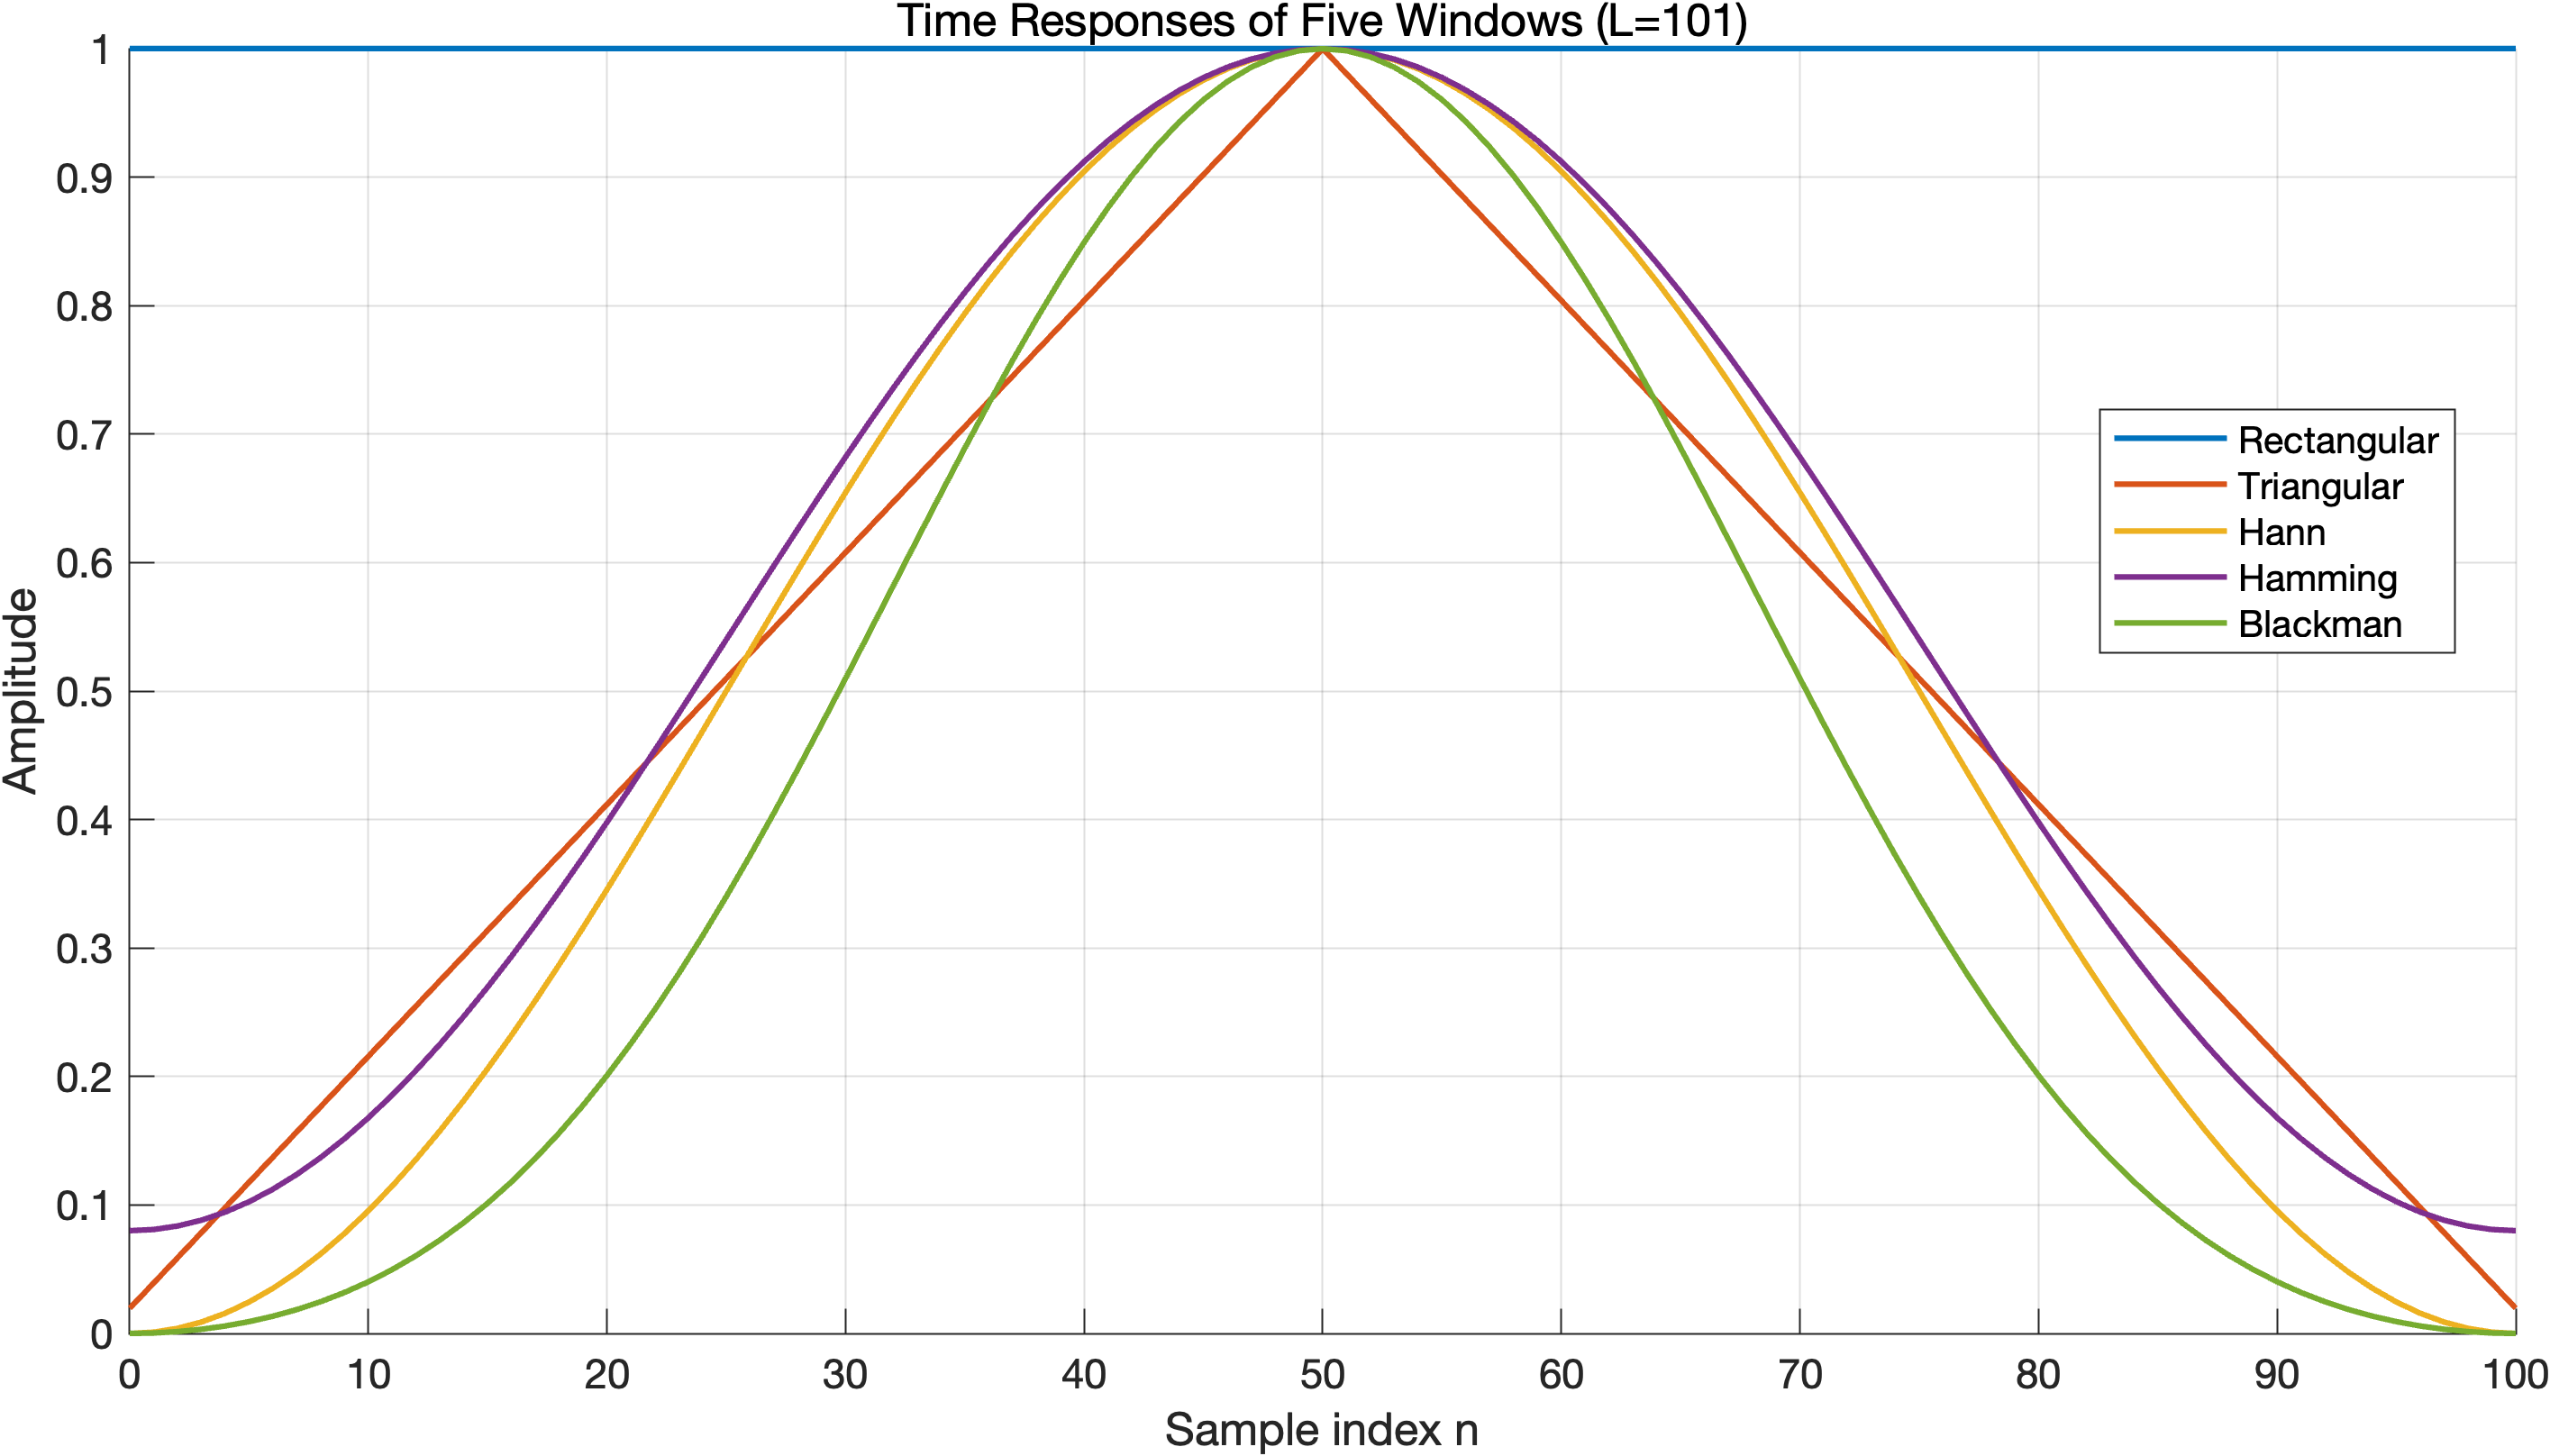
\includegraphics[width=0.86\textwidth]{figures/p1_time_windows.png}
    \caption{五种窗函数时域响应（$L=101$）}
    \label{fig:p1_time}
\end{figure}

\begin{figure}[H]
    \centering
    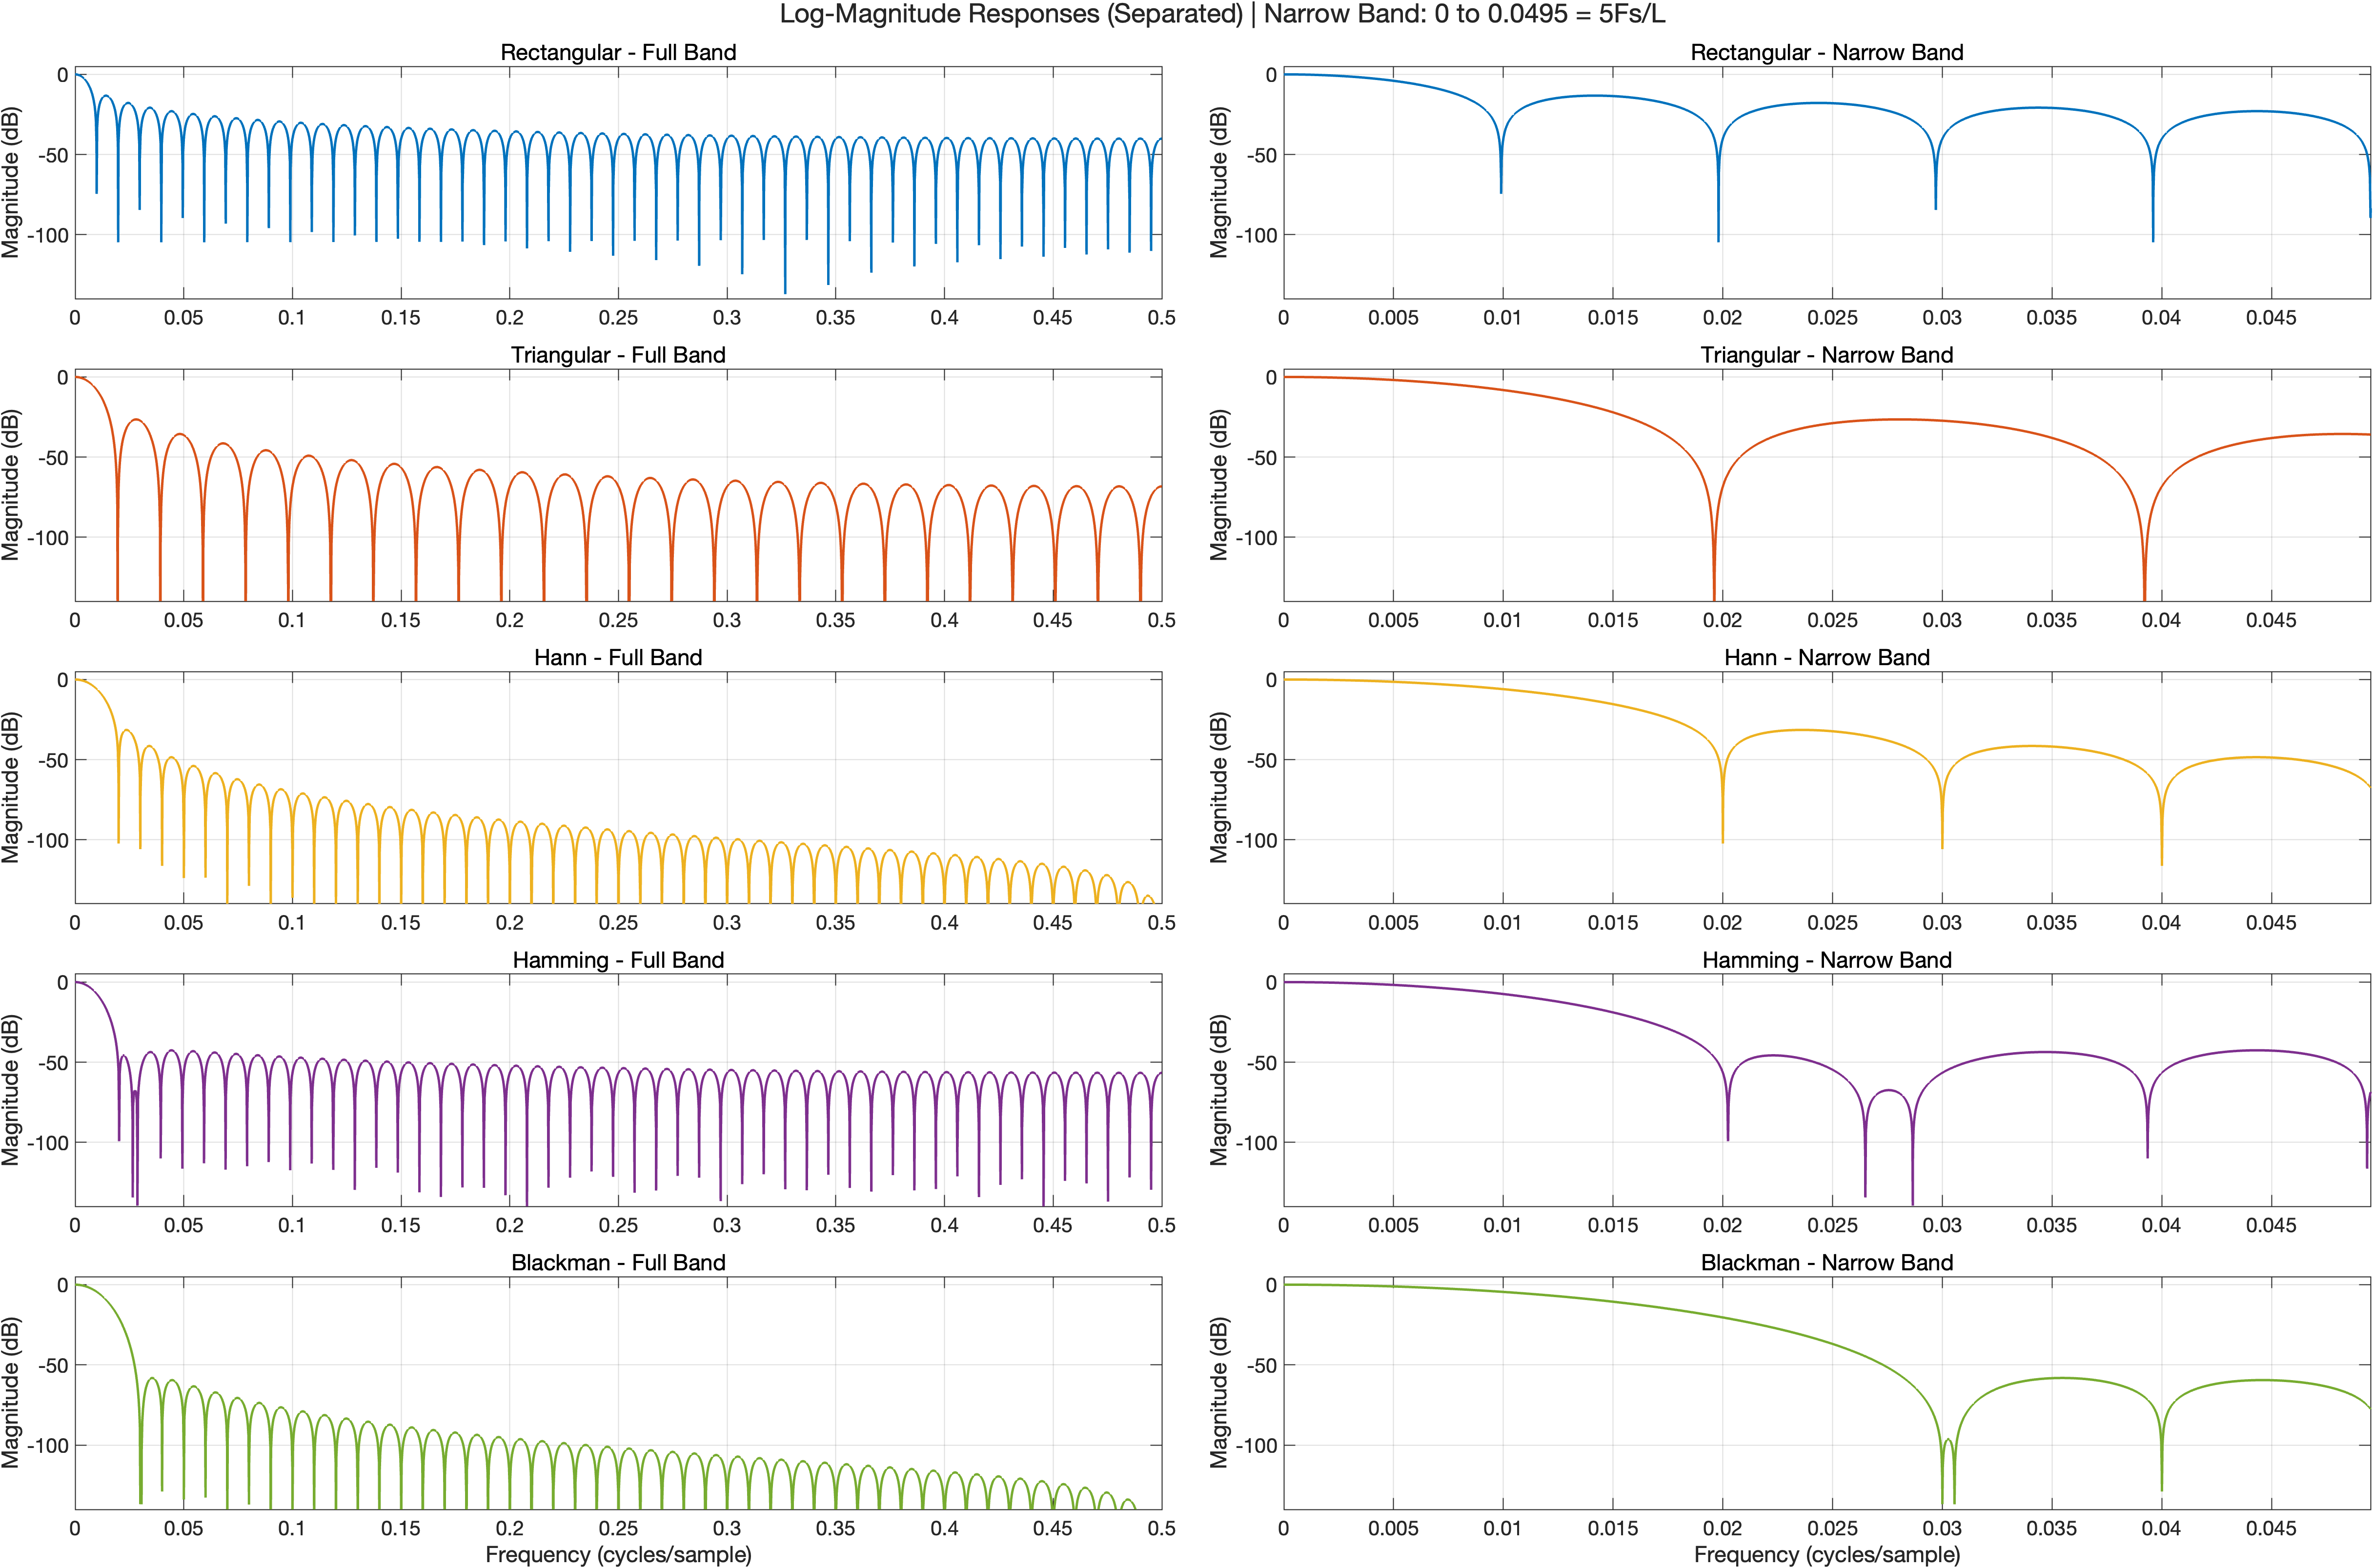
\includegraphics[width=\textwidth]{figures/p1_log_windows.png}
    \caption{五种窗函数频域对数幅度响应（分窗显示）}
    \label{fig:p1_freq}
\end{figure}

\subsubsection*{结果与回答}
根据计算结果，五种窗函数的有效带宽和峰值旁瓣电平见表~\ref{tab:p1_metrics}。

\begin{table}[H]
    \centering
    \caption{窗函数频域指标比较}
    \label{tab:p1_metrics}
    \begin{tabular}{lcc}
        \toprule
        窗函数 & 有效主瓣带宽（归一化频率） & 峰值旁瓣电平（dB） \\
        \midrule
        Rectangular & 0.0198 & -13.26 \\
        Triangular  & 0.0392 & -26.50 \\
        Hann        & 0.0400 & -31.47 \\
        Hamming     & 0.0405 & -42.58 \\
        Blackman    & 0.0600 & -58.11 \\
        \bottomrule
    \end{tabular}
\end{table}

针对题目要求可得结论：矩形窗主瓣最窄（带宽最小），但旁瓣最高，频谱泄漏最严重；Blackman 窗主瓣最宽，但旁瓣最低，抑制泄漏能力最强；Hann 与 Hamming 带宽相近，其中 Hamming 旁瓣更低，综合性能更均衡。

\subsection{Problem 2：语音短时特征分析}
\subsubsection*{题目要求}
对语音文件进行短时分析，并在同一页给出四项结果：原始波形、短时能量、短时幅值、短时过零率；同时说明窗长、帧移和窗型的选取依据。

\subsubsection*{实现方法}
设帧信号为
\begin{equation}
    x_n[m]=x[nR+m]w[m],\quad 0\le m\le L-1.
\end{equation}
对应三项短时特征定义为
\begin{align}
    E_n &= \sum_{m=0}^{L-1}|x_n[m]|^2,\\
    M_n &= \sum_{m=0}^{L-1}|x_n[m]|,\\
    Z_n &= \frac{1}{2}\sum_{m=1}^{L-1}\left|\operatorname{sgn}(x_n[m])-\operatorname{sgn}(x_n[m-1])\right|.
\end{align}
实验参数设置为 $L\approx20\,\mathrm{ms}$、$R\approx10\,\mathrm{ms}$（约 50\% 重叠）、Hamming 窗。测试文件使用 \texttt{s5.wav} 和 \texttt{test\_16k.wav}（正文图示以 \texttt{s5.wav} 为例）。该设置兼顾了短时平稳假设、时间分辨率和频谱泄漏抑制能力。

为满足题目“按采样率归一化尺度”的要求，时间轴统一采用 $t=n/f_s$（单位秒），不同语音文件分别使用各自采样率计算帧中心时刻；频率相关横轴采用归一化频率（cycles/sample）表示，使不同 $f_s$ 文件之间可直接比较。

\subsubsection*{关键代码段}
\begin{lstlisting}[caption={Problem 2：短时能量/幅值/过零率计算}]
for n = 1:numFrames
    idx0 = (n - 1) * R + 1;
    frame = x(idx0:idx0 + L - 1) .* window;

    energy(n) = sum(frame .^ 2);
    magnitude(n) = sum(abs(frame));

    s = sign(frame);
    s(s == 0) = 1;
    zc(n) = 0.5 * sum(abs(diff(s)));
end
\end{lstlisting}

\begin{figure}[H]
    \centering
    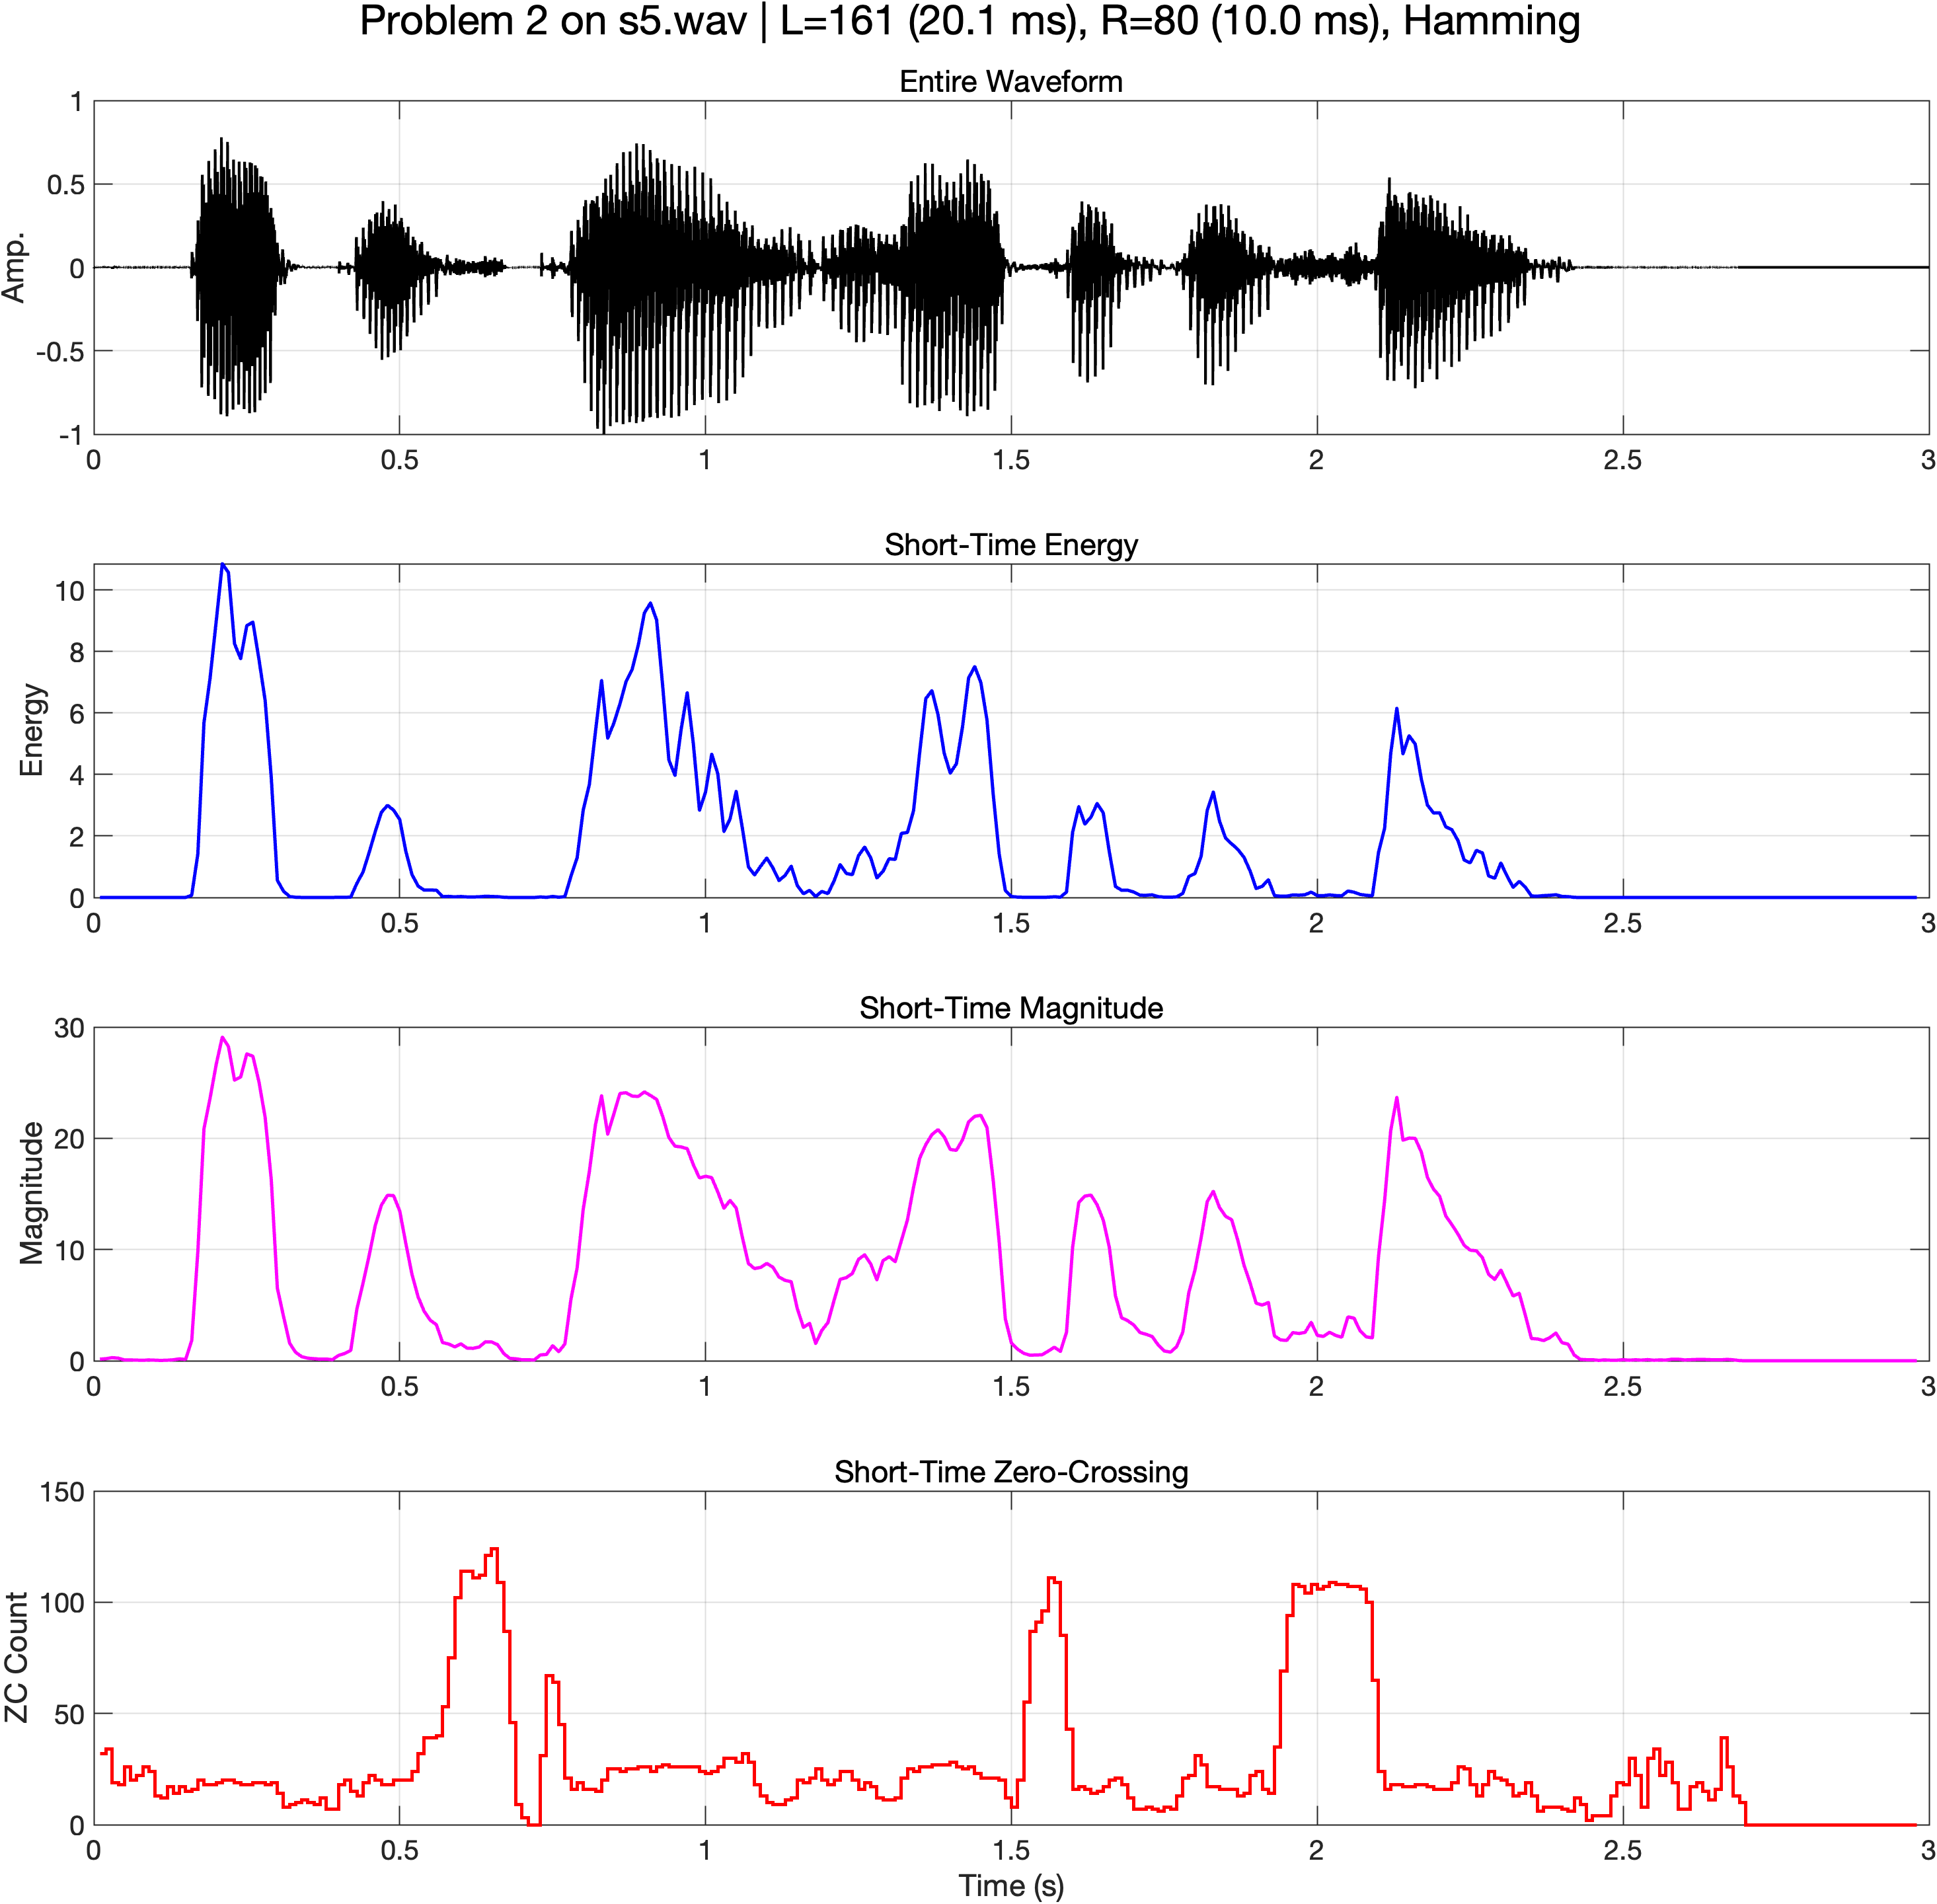
\includegraphics[width=0.95\textwidth]{figures/p2_short_time_features.png}
    \caption{语音波形与短时能量/幅值/过零率}
    \label{fig:p2_features}
\end{figure}

\subsubsection*{结果与回答}
从图~\ref{fig:p2_features} 可见，短时能量与短时幅值在时序上高度一致，峰值位置基本对应有声段；短时过零率在清音或高频噪声成分较强的区段明显升高。由此可回答题目：三项短时特征能够从“能量强弱”和“过零密度”两个互补角度描述语音结构，并支持有声段与清音段的区分。

\subsection{Problem 3：窗长对短时分析结果的影响}
\subsubsection*{题目要求}
在同一语音上比较不同窗长（$L=51,101,201,401$）时，短时能量、短时幅值和短时过零率的变化，并回答“窗长变短或变长后出现何种效应”。

\subsubsection*{实现方法}
语音文件选用 \texttt{test\_16k.wav}，窗函数取 Hamming。为保持接近 50\% 重叠，步长设为 $R=(L-1)/2$。为消除不同窗长带来的尺度偏置，本题比较时采用归一化特征：
\begin{align}
E_n^{(\mathrm{norm})} &= \frac{\sum_{m=0}^{L-1}|x_n[m]|^2}{\sum_{m=0}^{L-1}w^2[m]},\\
M_n^{(\mathrm{norm})} &= \frac{\sum_{m=0}^{L-1}|x_n[m]|}{\sum_{m=0}^{L-1}|w[m]|},\\
Z_n^{(\mathrm{norm})} &= \frac{0.5\sum_{m=1}^{L-1}\left|\operatorname{sgn}(x_n[m])-\operatorname{sgn}(x_n[m-1])\right|}{L-1}.
\end{align}
据此对每个窗长分别计算并叠加比较三类短时特征。

\subsubsection*{关键代码段}
\begin{lstlisting}[caption={Problem 3：多窗长归一化比较}]
Lset = [51, 101, 201, 401];
for k = 1:numel(Lset)
    L = Lset(k);
    R = (L - 1) / 2;
    win = hamming(L);
    feats = short_time_name(x, fs, R, win);

    eNorm = feats.energy ./ sum(win.^2);
    mNorm = feats.magnitude ./ sum(abs(win));
    zNorm = feats.zc ./ (L - 1);

    plot(ax1, feats.time, eNorm, 'DisplayName', sprintf('L=%d', L));
    plot(ax2, feats.time, mNorm, 'DisplayName', sprintf('L=%d', L));
    plot(ax3, feats.time, zNorm, 'DisplayName', sprintf('L=%d', L));
end
\end{lstlisting}

\begin{figure}[H]
    \centering
    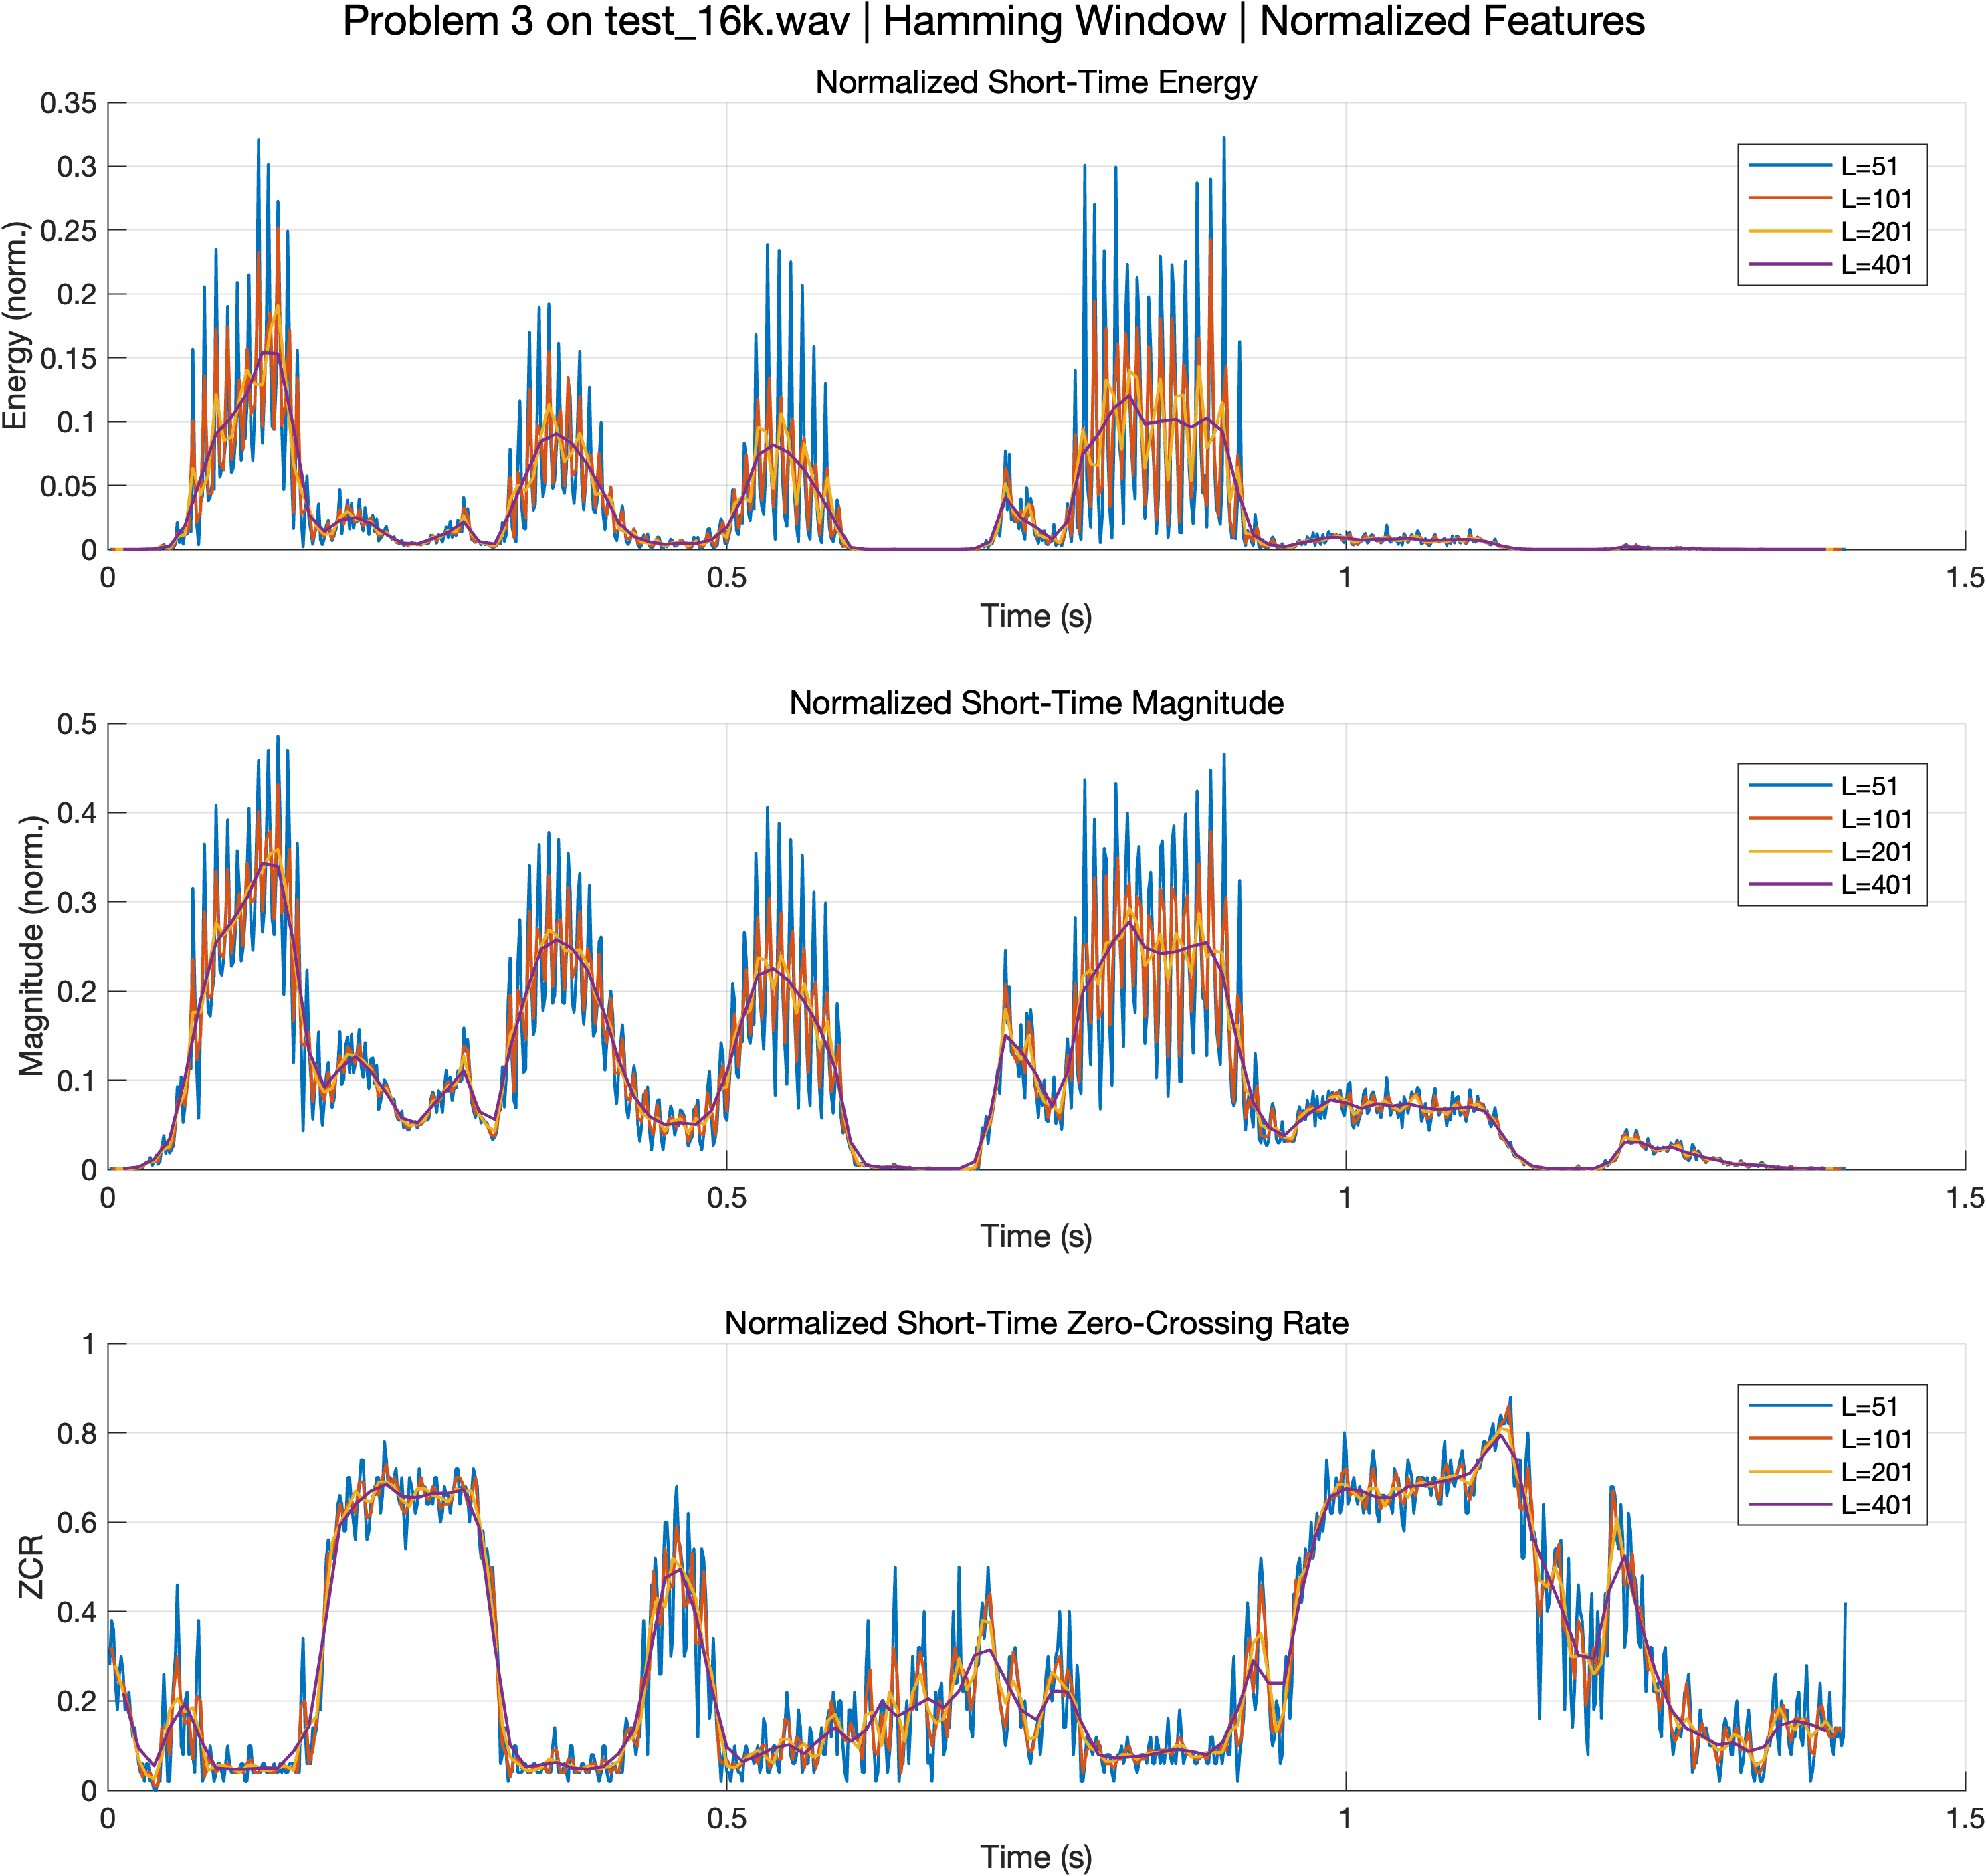
\includegraphics[width=0.95\textwidth]{figures/p3_window_length_effect.png}
    \caption{不同窗长下归一化短时特征对比}
    \label{fig:p3_compare}
\end{figure}

\subsubsection*{结果与回答}
图~\ref{fig:p3_compare} 表明，不同窗长下曲线差异主要体现在时间分辨率与平滑性之间的权衡。以本实验采样率 $f_s=16$\,kHz 为例，$L=51$ 对应窗口时长约为 $51/16000\approx3.2$\,ms，而 $L=401$ 对应约 $401/16000\approx25.1$\,ms。短窗（如 $L=51$）能够更敏感地响应局部快速变化，峰谷位置跟踪更及时，但曲线会出现更明显的高频抖动；这说明短窗保留了更多微观细节，同时也更易受瞬时扰动影响。长窗（如 $L=401$）对局部波动的平均作用更强，曲线轮廓更连续、语音包络更清晰，但瞬态细节会被削弱，快速起落边界被拉宽。可见，窗长增大等效于增强时间域平滑（可理解为更强的低通平均效应）；窗越长，稳定性越高而细节越少，窗越短则相反。该结果即为题目所要求的“窗长变短/变长效应”。

\section{结论}
本实验在统一短时分析框架下完成了三项验证。第一，窗函数存在“主瓣宽度—旁瓣抑制”权衡，矩形窗与 Blackman 窗分别对应两端，Hamming 窗表现出较好的综合折中。第二，短时能量、短时幅值与短时过零率可联合用于语音结构分析。第三，在归一化比较条件下，窗长主要影响短时估计的平滑程度与时间分辨率：长窗更平滑、短窗更敏感，实际应用中需按任务目标进行折中选取。


\end{document}
